\section{Section overview}
\begin{itemize}
    \item Sequence: So far what we've learned has been sequential programming, a series of statements running sequentially, our code can't make decisions.
    \item Selection structures: allow us to make decisions based on certain conditions being true or false.
    \item Iteration: looping or repeating.
\end{itemize}

With sequence, selection and iteration we can implement any algorithm.

\subsection{Selection: Decision}
\begin{itemize}
    \item \mintinline{cpp}{if} statement.
    \item \mintinline{cpp}{if else} statement.
    \item Nested \mintinline{cpp}{if} statements.
    \item \mintinline{cpp}{switch} statement.
    \item Conditional operator \mintinline{cpp}{?:;}
\end{itemize}

\subsection{Iteration: Looping}
\begin{itemize}
    \item \mintinline{cpp}{for} loop.
    \item Range-Based \mintinline{cpp}{for} loop.
    \item \mintinline{cpp}{while} loop.
    \item \mintinline{cpp}{continue} and \mintinline{cpp}{break}.
    \item Infinite loops.
    \item Nested loops.
\end{itemize}


%----------------------------------------------------------------------------------------
\section{If statement}
\begin{itemize}
    \item Syntax is: \verb|if (expr) { statement; }|.
    \item The control expression must evaluate to a boolean true or false value.
    \item If the expression is true then execute the statement.
    \item If the expression is false then skip the statement.
    \item As a recommendation we always indent the code inside the if statement.
\end{itemize}

\subsection{Examples of single if statements}
For single if statements you do not need to enclose the statements in curly braces.
\begin{figure}[H]
    \centering
    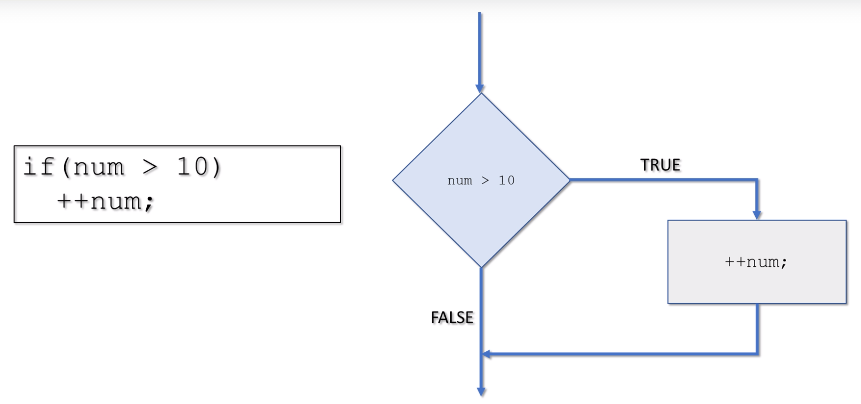
\includegraphics[width=0.4\textwidth]{./figs/single_if}
\end{figure}
\begin{minted}[autogobble]{cpp}
    if (selection == 'A')
        cout << "You selected A";
    if (num > 10)
        cout << "num is grater than 10";
    if (health < 100 && player_healed)
        health = 100;
\end{minted}

\subsection{Block if statements}
\begin{itemize}
    \item A block of code we have already seen in the main function.
    \item Create a block of code by including more than one statement in code block and adding \{\}.
    \item Blocks can also contain variable declarations.
    \item These variables are visible only within the block (local scope).
\end{itemize}
\begin{figure}[H]
    \centering
    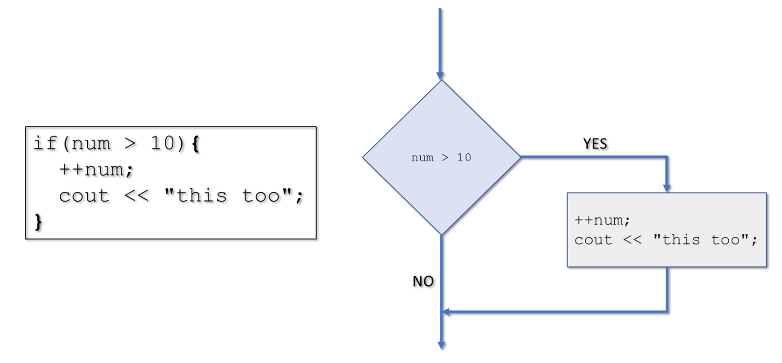
\includegraphics[width=0.4\textwidth]{./figs/multi_if}
\end{figure}

\subsection{Example of block ifs}
\begin{minted}[autogobble]{cpp}
    #include <iostream>
    using namespace std;
    int main() {
        int num {0};
        const int min {10}, max {100};
        cout << "Enter a number between " << min << " and " << max << ": ";
        cin >> num;
        if (num >= min) {
            cout << "\n================if statment 1===================" << endl;
            cout << num << " is grater than " << min << endl;
            int diff {num - min};
            cout << num << " is " << diff << " greater than " << min << endl;
        }

        if (num <= max) {
            cout << "\n================if statment 2===================" << endl;
            cout << num << " is less than or equal to " << max << endl;
            int diff {max - num};
            cout << num << " is " << diff << " less than " << max << endl;
        }

        if (num >= min && num <= max) {
            cout << "\n================if statment 3===================" << endl;
            cout << num << " is in range " << endl;
            cout << "This means statement 1 and 2 must also display!" << endl;
        }
        if (num == min || num == max) {
            cout << "\n================if statment 4===================" << endl;
            cout << num << " is in boundaries " << endl;
            cout << "This means statement 1, 2 and 3 must also display!" << endl;
        }
        return 0;
    }
    /* OUTPUT:
    Enter a number between 10 and 100: 100

    ================if statment 1===================
    100 is grater than 10
    100 is 90 greater than 10

    ================if statment 2===================
    100 is less than or equal to 100
    100 is 0 less than 100

    ================if statment 3===================
    100 is in range
    This means statement 1 and 2 must also display!

    ================if statment 4===================
    100 is in boundaries
    This means statement 1, 2 and 3 must also display!

    */
\end{minted}


%----------------------------------------------------------------------------------------
\section{If else statement}
\begin{itemize}
    \item Syntax:
        \begin{minted}[autogobble]{cpp}
            if (expr)
                statement;
            else
                statement2;
        \end{minted}
    \item If the expression is true then execute statement1.
    \item If the expression is false then execute statement2.
    \item Never forget the indentation.
\end{itemize}
\begin{figure}[H]
    \centering
    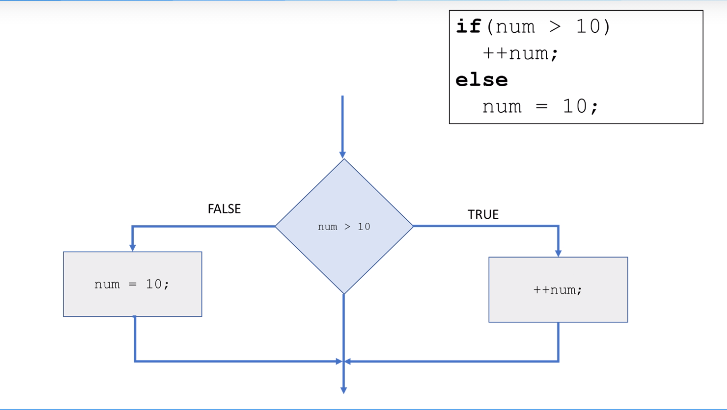
\includegraphics[width=0.4\textwidth]{./figs/ifelse}
\end{figure}

\subsection{Example of single if else statements}
\begin{minted}[autogobble]{cpp}
    if (num > 10)
        cout << "num is greater than 10";
    else 
        cout << "num is NOT greater than 10";
    
    if (health < 100 && heal_player) 
        health = 100;
    else 
        ++health;
\end{minted}


\subsection{If else block}
\begin{figure}[H]
    \centering
    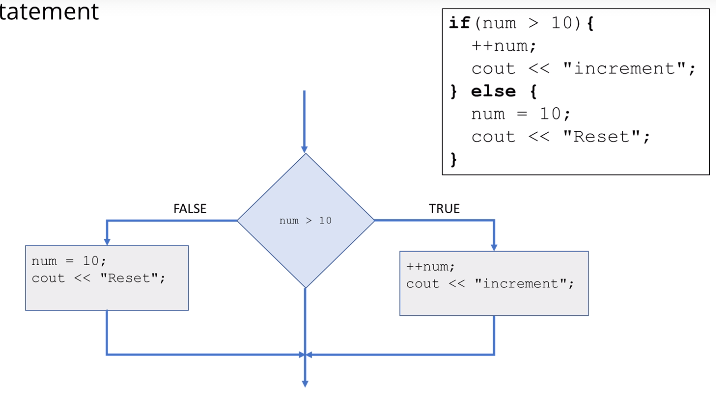
\includegraphics[width=0.4\textwidth]{./figs/multiifelse.png}
\end{figure}


\subsection{If else if construct}
\begin{itemize}
    \item Sometimes we need to check multiple conditions not just weather the expression is true but other characteristics, for this we use an if else if construct.
\end{itemize}
\begin{minted}[autogobble]{cpp}
    if (score > 90)
        cout << "A";
    else if (score > 80)
        cout << "B";
    else if (score > 70)
        cout << "C";
    else if (score > 60)
        cout << "D";
    else
        cout << "F";
    cout << "Done";
\end{minted}

\subsection{Example}
\begin{minted}[autogobble]{cpp}
    #include <iostream>
    using namespace std;
    int main() {
        int num{};
        const int target {10};
        cout << "Enter a number and I'll compare it to " << target << ": ";
        cin >> num;

        if (num >= target) {
            cout << "\n==========================" << endl;
            cout << num << " is greater than or equal to " << target << endl;
            int diff {num - target};
            cout << num << " is " << diff << " greater than " << target << endl;
        } else {
            cout << "\n==========================" << endl;
            cout << num << " is less than " << target << endl;
            int diff {target - num};
            cout << num << " is " << diff << " less than " << target << endl;
        }
        cout << endl;
        return 0;
    }
    /* OUTPUT:
    Enter a number and I'll compare it to 10: -10

    ==========================
    -10 is less than 10
    -10 is 20 less than 10

    */
\end{minted}


%----------------------------------------------------------------------------------------
\section{Nested if statement}
\begin{itemize}
    \item You can nest if statements within other if statements.
        \begin{minted}[autogobble]{cpp}
            if (expr1) 
                if (expr2) 
                    statement1;
                else 
                    statement2;
        \end{minted}
    
    \item If the expression is true then execute statement1.
    \item If the expression is false then execute statement2.
    \item Many times we need more logic to the if statement.
    \item In the above example the if statement expects one statement without the curly braces, however the if statement is a one compound statement and that is why the above code doesn't need curly braces.
    \item Notice, how does the computer know if the else statement belongs to the closest or farthest if? In C++ each else belogs to the closest if, so in the above example it belongs to the if holding the expr2.
    \item Remember to indent.
\end{itemize}

\subsection{Example}
\begin{itemize}
    \item Example of scores:
        \begin{minted}[autogobble]{cpp}
            if (score > 90) 
                if (score > 95)
                    cout << "A+";
                else 
                    cout << "A";
            cout << "Sorry, No A";
        \end{minted}
        \begin{figure}[H]
            \centering
            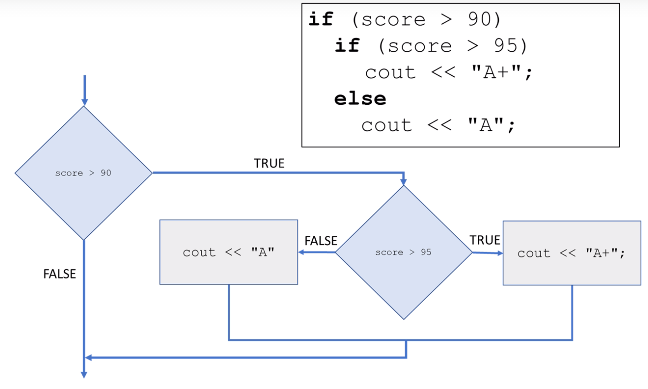
\includegraphics[width=0.4\textwidth]{./figs/exnestedif.png}
        \end{figure}
    
    \item Example:
        \begin{minted}[autogobble]{cpp}
            if (score_frank != score_bill) {
                if (score_frank > score_bill) {
                    cout << "Frank wins" << endl;
                } else {
                    cout << "Bill wins" << endl;
                }
            } else {
                cout << "Looks like a tie!" << endl;
            }
        \end{minted}
    
    \item Example of nested latter:
        \begin{minted}[autogobble]{cpp}
            #include <iostream>
            using namespace std;
            int main() {
                int score {};
                cout << "Enter your score in the exam (0-100): ";
                cin >> score;
                char letter_grade {};

                if (score >= 0 && score <= 100) {
                    if (score >= 90)
                        letter_grade = 'A';
                    else if (score >= 80)
                        letter_grade = 'B';
                    else if (score >= 70)
                        letter_grade = 'C';
                    else if (score >= 60)
                        letter_grade = 'D';
                    else
                        letter_grade = 'F';
                    cout << "Your grade is: " << letter_grade << endl;
                    if (letter_grade == 'F') 
                        cout << "Bad grade." << endl;
                    else 
                        cout << "Congrats." << endl;
                } else {
                    cout << "Sorry, " << score << "is not in range." << endl;
                }
                return 0;
            }
            /* OUTPUT:
            Enter your score in the exam (0-100): 90
            Your grade is: A
            Congrats.

            */
        \end{minted}
\end{itemize}


%----------------------------------------------------------------------------------------
\section{Switch-case statement}
